\documentclass[cfonts,nofontsdir]{nostarch}
\usepackage{lipsum}
\hyphenation{ve-sti-bu-lum sene-c-tus rut-rum con-sec-te-tu-er
  elei-fend no-num-my li-be-ro}
\usepackage{natbib}
\usepackage{nshyper}
\lstset{fancyvrb=true}
\usepackage{amsmath}
\makeindex
\begin{document}


\frontmatter

\author{Boris Veytsman}

\title{\emph{No Starch Press} example file}

\subtitle{A short demonstration}

\nostarchlogo{vitruvian.jpg}

\makehalftitle

\maketitle


\begin{copyrightpage}
  \textbf{\sffamily\MakeUppercase{\emph{No Start Press} example file}}
  Copyright \textcopyright{} 2023 by Boris Veytsman

  No rights reserved. Any part of this work may be reproduced or
  transmitted in any form or by any means, electronic or mechanical,
  including photocopying, recording, or by any information storage or
  retrieval system, without the prior written permission of the
  copyright owner and the publisher.

  \raisebox{-8pt}{
\includegraphics[height=20pt]{recycled}} Typeset
  with recycled electrons in the United States of America

11 10 09 08 07 \hspace{0.5in}  123456789\\
ISBN-10: 1-23456-789-0\\
ISBN-13: 123-4-56789-012-3

Publisher: P.~U.~Blisher\\
Production Editor: E.~D.~Itor\\
Cover and Interior Design: Calamari Studios\\
Developmental Editor: D.~E.~Itor\\
Technical Reviewer: R.~E.~Viewer\\
Copyeditor: C.~O.~Editor\\
Compositor: A.~U.~Thor\\
Proofreader: P.~R.~\O freader\\
Indexer: I.~N.~Dexer

For information on book distributors or translations, please contact
No Starch Press, Inc. directly: \\
No Starch Press, Inc.\\
555 De Haro Street, Suite 250, San Francisco, CA 94107\\
phone: 415.863.9900; fax: 415.863.9950; info@nostarch.com; www.nostarch.com\\

\begin{cipblock}
Uthor, A. U. and Respondent, C. O. R. and Iter, W. R.
  Pellentesque habitant morbi: Cum sociis natoque penatibus/
  A. U. Thor, C. O. R. Respondent and W. R. Iter
       p. cm.
  Includes index.
  ISBN-10: 1-23456-789-0
  ISBN-13: 123-4-56789-012-3
  1.  Morbi (habitant).  2. Penatibus. I. Title.
XX2303.5.T324 2008
\end{cipblock}

No Starch Press and the No Starch Press logo are registered trademarks
of No Starch Press, Inc. Other product and company names mentioned
herein may be the trademarks of their respective owners. Rather than
use a trademark symbol with every occurrence of a trademarked name, we
are using the names only in an editorial fashion and to the benefit of
the trademark owner, with no intention of infringement of the
trademark.

The information in this book is distributed on an ``As Is'' basis,
without warranty. While every precaution has been taken in the
preparation of this work, neither the author nor No Starch Press, Inc.
shall have any liability to any person or entity with respect to any
loss or damage caused or alleged to be caused directly or indirectly
by the information contained in it.


\end{copyrightpage}

\begin{dedicationpage}
  God of the golden bow,\\
      And of the golden lyre,\\
And of the golden hair,\\
      And of the golden fire,\\
            Charioteer\\
            Of the patient year,\\
      Where---where slept thine ire,\\
When like a blank idiot I put on thy wreath,\\
      Thy laurel, thy glory,\\
      The light of thy story,\\
Or was I a worm---too low crawling for death?\\
      O Delphic Apollo!

\bigskip
\emph{John Keats}
\index{Keats, John@\emph{Keats, John}}
\index{gods!Greek!Apollo}
\index{Apollo|see{gods, Greek}}
\index{Greek gods|see{gods, Greek}}
\end{dedicationpage}

\brieftableofcontents

\tableofcontents

\chapter*[Foreword by R.~E.~Viewer]{Foreword}

This is a foreword.  Note that the chapter\index{chapter} has two
arguments: the title of the chapter and the title for the table of
contents\index{table of contents!adding to}.  The first paragraph
is automatically typeset in a larger font.

Now a couple of paragraphs of filler text to make some pages.

\lipsum[1-3]

\bigskip

\begin{raggedright}
\bfseries
R.~E.~Viewer\index{Viewer, R. E.@\emph{Viewer, R.~E.}}\\
New York\index{USA!states!New York}\index{New York|see{USA, states}}\\
December 2007
\end{raggedright}

\mainmatter
\part{The first part}

The main part of the book starts with the command, well,
\path{\mainmatter}\index{main matter}.

Again some filler.

\lipsum[77-78]

\chapter[The first chapter]{The first chapter (the long title)}

\chapterartfile{1eurogr}\index{euro, coin!Greece}\index{Greek euro|see{euro}}

The first chapter again has two versions of the title.  There is a
special command \path{\chapterartfile}.  It adds the art vignette to
the start of the chapter.  Now again some filler---but here we show
how to add index entries to the text.  Fusce adipiscing justo nec
ante. Nullam in enim.  Pellentesque felis orci, sagittis ac, malesuada
et, facilisis in, ligula\index{ligula}.  Nunc\index{nunc} non magna
sit amet mi aliquam dictum\index{dictum}.

\section{Quisque aliquam ipsum sed turpis}

Some additional filler\ldots


\lipsum[1]

Nam dui ligula\index{ligula}, \emph{fringilla a}, euismod sodales,
sollicitudin vel, wisi.  Morbi auctor lorem non justo. Nam lacus
libero, pretium at, lobortis vitae\index{vita}, ultricies et, tellus.
Donec \textbf{aliquet,} tortor sed accumsan bibendum, erat
ligula\index{ligula} aliquet magna, vitae\index{vita} ornare odio
metus a mi.

Morbi ac orci et nisl hendrerit mollis.  Proin tellus est, luctus
vitae\index{vita}, molestie a, mattis et, mauris. Donec tempor. Pellentesque
habitant morbi tristique senectus et netus et malesuada fames ac
turpis egestas. Duis ante felis, dignissim id, blandit in, suscipit
vel, dolor.  Suspendisse ut massa. Cras nec ante\footnote{\lipsum[4]}.
\texttt{{\itshape Pellentesque} a nulla.}  Cum sociis natoque
penatibus et magnis dis parturient montes, nascetur ridiculus mus.
Aliquam tincidunt urna.  Nulla ullamcorper vestibulum turpis.
Pellentesque cursus luctus mauris\footnote{\lipsum[3]}.

\lipsum[10]

\section{Nunc\index{nunc} non magna sit amet mi aliquam dictum}

The index can be even in the section head.

\lipsum[32-33]

\subsection{Nam sed augue}

\lipsum[34-35]

\subsubsection{Pellentesque tincidunt cursus felis}

\lipsum[36-38]

\chapter{Footnotes, figures and tables}
\label{chap:proin}
\chapterartfile{100euroit}\index{euro, coin!Italy}\index{Italian
  euro|see{euro}} 


Some examples of footnotes.  Aenean imperdiet\footnote{Quisque aliquam
  ipsum sed turpis\index{turpis}}.  Vestibulum ante ipsum pri\-m\-is
in faucibus orci luctus et ultrices posuere cubilia Curae; Donec
lacinia nonummy lectus. Proin vel urna.  Fusce sit amet orci ac magna
iaculis pharetra.

Fusce adipiscing justo nec ante. Nullam in enim.  Pellentesque felis
orci, sagittis ac, malesuada et, facilisis in, ligula\index{ligula}.
Nunc\index{nunc} non magna sit amet mi aliquam dictum. In mi.
Curabitur sollicitudin justo sed quam. Aenean imperdiet.
\begin{enumerate}
\item Aenean adipiscing auctor est.
\item Morbi quam arcu, malesuada sed, volutpat et, elementum sit
  amet, libero.  Duis accumsan.
\item Curabitur urna.
\item In sed ipsum.
\end{enumerate}

Maecenas enim\index{enim!Maecenas}. Proin quis neque nec tortor
sollicitudin volutpat.  Sed at ante. Sed vitae\index{vita} mauris non
ante egestas hendrerit.  Cum sociis natoque penatibus et magnis dis
parturient montes, nascetur ridiculus mus. In
venenatis\index{venenatis} facilisis magna\index{magna}. Phasellus
purus. Cras quis mauris.  Aliquam eget magna. Donec rutrum sagittis
mi. Morbi elementum, est sit amet sollicitudin feugiat, orci magna
semper risus, eu congue nulla metus vel elit. Nunc\index{nunc} tempor
ornare mi.  Integer justo odio, suscipit tincidunt, fermentum eu,
tincidunt\index{tincida} et, libero.  Vestibulum vestibulum, urna et
suscipit imperdiet, nulla ante fermentum erat, at laoreet lorem lectus
sed metus. Fusce ante sem, posuere in, vehicula a, posuere sed, ante.
Phasellus magna.  Maecenas sit amet diam.  Nunc\index{nunc} at nibh
sit amet augue tristique gravida.\index{ante}
\begin{itemize}
\item Donec lobortis nibh.
\item Duis mattis.
\item Sed cursus lectus quis odio.
\item Phasellus arcu.
\item Praesent imperdiet dui in sapien\index{sapien}.
\item Vestibulum tellus pede, auctor a, pellentesque sit amet, vulputate sed,
  purus.
\item Nunc\index{nunc} pulvinar, dui at eleifend adipiscing, tellus
  nulla placerat massa, sed condimentum nulla tellus sed
  ligula\index{ligula}. Nulla vitae\index{vita} odio sit amet leo
  imperdiet blandit. In vel massa. Maecenas varius dui at turpis. Sed
  odio.
\end{itemize}


\begin{figure}[tp]
  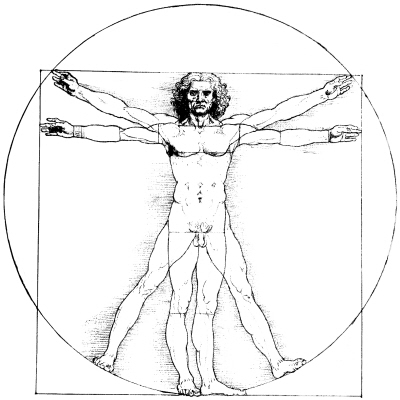
\includegraphics[width=3in]{vitruvian}
  \index{Da Vinci, Leonardo@\emph{Da Vinci, Leonardo}}
  \index{Leonardo Da Vinci@\emph{Leonardo Da Vinci}|see{Da Vinci,
      Leonardo}}
  \index{Vitruvian Man}
  \caption{Vitruvian man.  Note that the caption is typeset in a box
    with the width automatically calculated from the image.}
  \label{fig:one}
\end{figure}


\section{Donec vel augue}


Donec\index{donec|(} vel augue. Morbi a turpis sed libero consequat
porta. Quisque lacinia consequat odio. Sed vehicula sollicitudin
purus. Vestibulum eget est. In hac habitasse platea dictumst. Sed
blandit, tortor a auctor imperdiet, wisi nibh ornare leo, ac dictum
nibh enim eu orci.  Pellentesque habitant morbi tristique senectus et
netus et malesuada fames ac turpis egestas.  Aliquam tincidunt
ullamcorper justo. Etiam accumsan lacus nec ante.  Ut dictum luctus
mauris. Ut metus. Maecenas gravida. Proin iaculis.  Integer convallis,
justo iaculis ullamcorper sollicitudin, lectus neque tincidunt mi, at
condimentum sem quam vel diam. Aenean sit amet purus.
\begin{quote}
  Nam quis ante. Nullam interdum quam in eros.  Sed eleifend libero eu
  tellus consequat fermentum. Nullam pellentesque risus ut augue.
  Vestibulum eu tellus. Integer eleifend suscipit urna. Fusce
  porttitor leo et odio. Vivamus vehicula justo a nisl. In rutrum,
  purus ut dictum auctor, dolor velit accumsan dolor, eu convallis
  augue dui ac lectus. 
\end{quote}

Vestibulum at lectus. Vestibulum dapibus placerat magna. Suspendisse
dolor urna, condimentum sit amet, euismod a, adipiscing a, enim.
Aliquam erat volutpat. Donec imperdiet dolor non mi. Phasellus magna
metus, dictum sit amet, laoreet non, dictum vel, dui. Suspendisse
potenti. Nunc\index{nunc} turpis risus, porta vel, pharetra id,
eleifend vitae\index{vita}, justo. Duis pulvinar dolor sit amet urna.
Integer eu eros. Nulla facilisi. Duis dui.  Nullam vitae\index{vita}
quam. Morbi a nunc\index{nunc} in elit sodales euismod.
Nunc\index{nunc} sed orci. Etiam malesuada metus vitae\index{vita}
felis. Suspendisse imperdiet velit in tellus.
\begin{quotation}
\lipsum[40-41]  
\end{quotation}
\lipsum[63-65]
\begin{Code}[commandchars=\\\[\]]
\textit[/* S.C. Johnson, B.W. Kernighan, The Programming Language B, 1972 */]
main( ) {
   extrn a, b, c;
   putchar(a); putchar(b); putchar(c); putchar('!*n');
 }
 a 'hell';
 b 'o, w';
 c 'orld';  
\end{Code}
\index{Johnson, S.~C.@\emph{Johnson, S.~C.}}
\index{Kernigan, B.~W.@\emph{Kernigan, B.~W.}}
\index{B|see{programming languages}}
\index{programming languages!B}
\index{operators!putchar@\texttt{putchar}}
\index{putchar@\texttt{putchar}|see{operators}}
\index{operators!extrn@\texttt{extrn}}
\index{extrn@\texttt{extrn}|see{operators}}
\index{functions!main@\texttt{main}}
\index{main@\texttt{main}|see{functions}}
\index{()@\texttt{( )} (parentheses)}
\index{{}@\texttt{\{ \}} (braces)}
\index{/*@\texttt{/*} (comment start)}
\index{*/@\texttt{*/} (comment end)}
\index{;@\texttt{;} (semicolon)}


\begin{lstlisting}[language=Lisp, frame=single, float,
  caption={[Hello, World in Emacs
  Lisp]Hello, World in Emacs Lisp%
    \index{Lisp|see{programming languages}}%
    \index{programming languages!Lisp}\index{Emacs}}] 
;;; Hello World in Emacs Lisp.

(defun hello-world()
  "Display the string hello world."
  (interactive)
  (message "hello world"))
\end{lstlisting}

Integer posuere, metus ac rhoncus auctor, mi tellus scelerisque
nunc\index{nunc}, venenatis elementum tortor lorem eu erat.
\begin{description}
\item[Sed:] consectetuer risus vitae\index{vita} orci. Nullam tortor
  mauris, interdum at, imperdiet in, convallis eget, massa.
\item[Aliquam:] suscipit, magna nec blandit volutpat, lectus neque
  suscipit nunc\index{nunc}, sit amet cursus nisl erat eget risus.
  Vestibulum leo lectus, accumsan ut, pharetra vel, elementum sed,
  quam. Maecenas condimentum orci at enim. Maecenas ut
  nunc\index{nunc}. Vivamus pede. Integer vel purus vel mi mollis
  vestibulum. Sed laoreet ultricies nibh.  Suspendisse non nisl quis
  ligula\index{ligula} fermentum facilisis.
\end{description}
\lipsum[37]


\begin{table}[tp]
  \caption[Sed blandit, tortor a auctor]{Sed blandit, tortor a auctor
    imperdiet, wisi nibh ornare leo, 
    ac dictum nibh enim eu orci}
  \begin{tabular}{lll}
    \toprule
    \thfont Phasellus &  \thfont At Dui       & \thfont Donec Commodo \\
    \midrule    
     Augue At Nunc    & Nunc In  sapien       & Et magna mollis \\
     Sagittis         &  Morbi eu elit        &  Phasellus lacus\\
     Donec a quam     & Etiam pulvinar sapien & Sed nibh magna\\
    \bottomrule
  \end{tabular}
\label{tab:one}
\end{table}

\lipsum[60]

Curabitur hendrerit. Morbi fringilla enim quis nunc\index{nunc}.
Phasellus at dui. Curabitur fringilla dui a odio.  Nunc\index{nunc}
semper condimentum arcu.
\begin{note}
  Donec commodo augue at nunc\index{nunc}. Nunc\index{nunc} in
  sapien\index{sapien} et magna mollis sagittis. Morbi eu elit.
  Phasellus lacus.  Donec a quam. Etiam pulvinar sapien\index{sapien}.
  Sed nibh magna, viverra vitae\index{vita}, auctor eget, eleifend
  nec, lorem.
\end{note}
Curabitur vitae\index{vita} lectus sit amet turpis pretium
condimentum. Nullam imperdiet mattis neque. Proin eget magna porta
erat rhoncus consectetuer. Aenean pulvinar erat vitae\index{vita} mi.
\index{donec|)}


\section{Proin eget magna porta erat rhoncus consectetuer}

\lipsum[123-125]

\begin{longtable}{lll}
  \caption{This is a longtable with a very long caption. It will be
    typeset in several lines}\label{tab:longtable}\\
  \toprule
  \thfont First column & \thfont Second column\\
  \midrule
  \endfirsthead
  \caption[]{This is a longtable with a very long caption. It will be
    typeset in several lines---continued\ldots}\\
  \toprule
  \thfont First column & \thfont Second column\\
  \midrule
  \endhead
  \bottomrule
  \endfoot
  a & b\\
  ab & bc\\
  $\alpha$ & $\beta$\\
  a & b\\
  ab & bc\\
  $\alpha$ & $\beta$\\
  a & b\\
  ab & bc\\
  $\alpha$ & $\beta$\\
  a & b\\
  ab & bc\\
  $\alpha$ & $\beta$\\
  a & b\\
  ab & bc\\
  $\alpha$ & $\beta$\\
  a & b\\
  ab & bc\\
  $\alpha$ & $\beta$\\
\end{longtable}


\part{Curabitur vitae}\index{vita|(}
\label{part:Curabitur}

\chapter[Curabitur vitae lectus]{Curabitur vitae lectus sit amet
  turpis pretium condimentum}

\chapterart{
\includegraphics[width=1.264in]{100euroie}}
\index{euro, coin!Ireland}\index{Irish euro|see{euro}} 



\lipsum[43-48]

\section{Sed blandit, tortor a auctor imperdiet, wisi nibh ornare leo,
  ac dictum nibh enim eu orci}

\lipsum[94-98]
\index{vita|)}

\backmatter

\nocite{*}
\bibliographystyle{plainnat}
\bibliography{nostarch}

\printindex

\updatespage

Visit \url{http://borisv.lk.net/latex.html} for updates, errata, and
other information.


\colophon

The book was produced as an example of the package \texttt{nostarch}. 

\end{document}
